\documentclass[12pt,a4paper,openright, notitlepage]{report}

% l'interlinea
\linespread{1.4}
\setlength{\parskip}{0.3cm plus4mm minus3mm} % spazio verticale paragrafi

\usepackage[italian]{babel} % Italian language
\usepackage[utf8x]{inputenc} % utf8

\usepackage[T1]{fontenc} % Use 8-bit encoding that has 256 glyphs
\usepackage{fourier} % Use the Adobe Utopia font

\usepackage{graphicx}
\usepackage{wrapfig}
\usepackage{subfigure}
\usepackage{changepage}

\usepackage{url}

\usepackage{amsmath,amsfonts,amsthm} % Math packages

\usepackage{sectsty} % Allows customizing section commands
\allsectionsfont{ \normalfont\scshape} % Make all sections centered, the default font and small caps

\usepackage{fancyhdr} % Custom headers and footers
\pagestyle{fancyplain} % Makes all pages in the document conform to the custom headers and footers
\fancyhead{} % No page header - if you want one, create it in the same way as the footers below
\fancyfoot[L]{} % Empty left footer
\fancyfoot[C]{} % Empty center footer
\fancyfoot[R]{\thepage} % Page numbering for right footer
\renewcommand{\headrulewidth}{0pt} % Remove header underlines
\renewcommand{\footrulewidth}{0pt} % Remove footer underlines
\setlength{\headheight}{13.6pt} % Customize the height of the header

\usepackage[font=small,labelfont=bf]{caption} %Style of the caption of figures
\usepackage{float} %to force the figure position

\setlength\parindent{0pt} % Removes all indentation from paragraphs

% Style dell'abstract
\usepackage{abstract}

%----------------------------------------------------------------------------------------
% TITLE
%----------------------------------------------------------------------------------------

\newcommand{\horrule}[1]{\rule{\linewidth}{#1}}

\title{	
\normalfont \normalsize 
\textsc{Università degli studi di Bologna} \\ [25pt]
\horrule{0.5pt} \\[0.4cm]
\huge Visual Directions Tests \\
\horrule{2pt} \\[0.5cm]
}

\author{Andrea Aquino, Matteo Brucato, Miro Mannino}

\date{\normalsize\today}

\begin{document}

\maketitle

%----------------------------------------------------------------------------------------
%----------------------------------------------------------------------------------------

\newpage

Look at the video. The test supervisor will show you. \\
You are watching a video about a path. You can watch the video several times. \\
You should watch the video until you feel confident enough to go the path on your own \textbf{in real life}.  \\
Afterwards we will ask you some easy question. \\
You can ask the test supervisor for any question. \\

We ask you some information about you. \\
Its up to you how much information you want to provide us. \\

\begin{itemize}
	\item Sex: 
	\item Age: 
	\item Nationality:
	\item Study field:
\end{itemize}

	
\newpage

\subsection{Question 1.1}

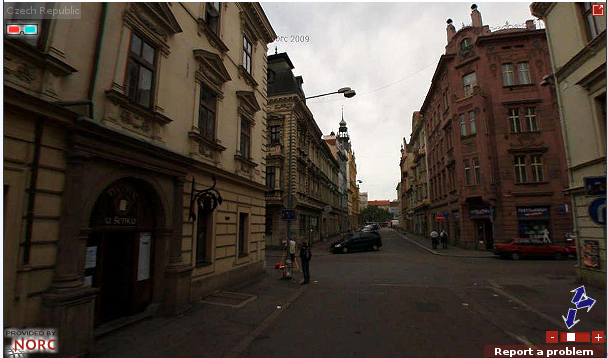
\includegraphics[width=\textwidth]{imgs/image-question11-1}

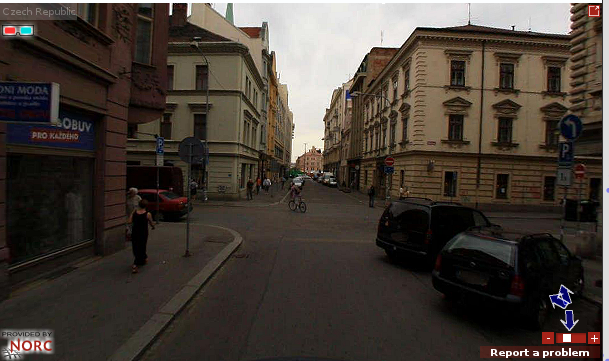
\includegraphics[width=\textwidth]{imgs/image-question11-2}

\begin{itemize}
	\item Do you recognize this point of the city?
	\item If you recognize it, where should you go in order to reach the destination you saw in the video?
\end{itemize}


\newpage

\subsection{Question 1.2}

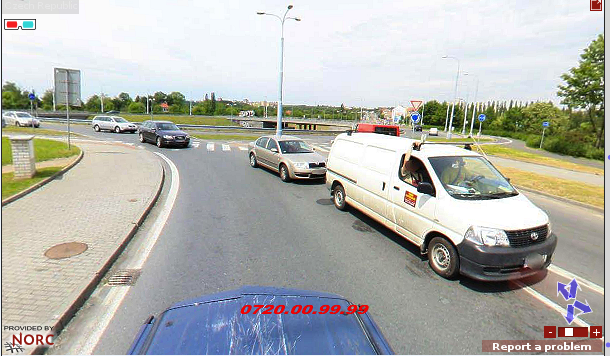
\includegraphics[width=\textwidth]{imgs/image-question12-1}
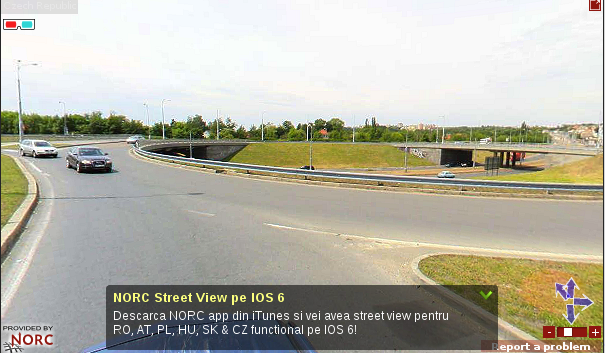
\includegraphics[width=\textwidth]{imgs/image-question12-2}

\begin{itemize}
	\item Do you recognize this point of the city?
	\item If you recognize it, where should you go in order to reach the destination you saw in the video?
\end{itemize}

\newpage

\subsection{Question 1.3}

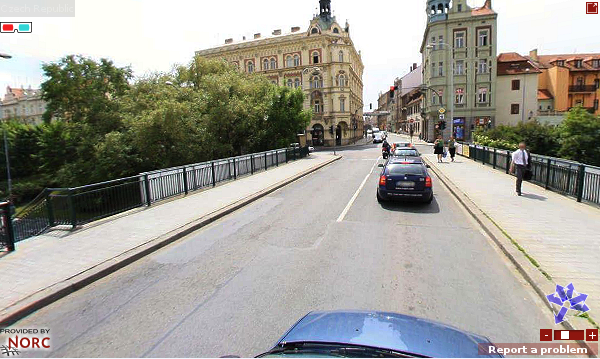
\includegraphics[width=\textwidth]{imgs/image-question13-1}
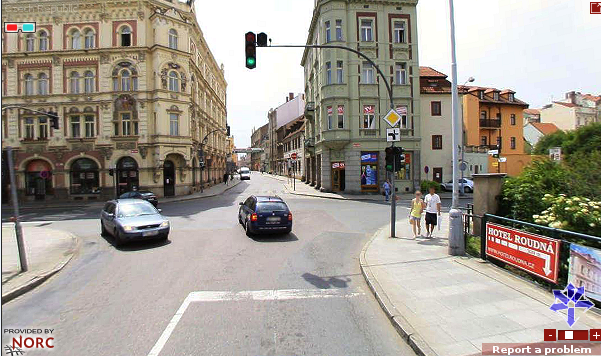
\includegraphics[width=\textwidth]{imgs/image-question13-2}

\begin{itemize}
	\item Do you recognize this point of the city?
	\item If you recognize it, where should you go in order to reach the destination you saw in the video?
\end{itemize}

\newpage

\subsection{Question 2.1}

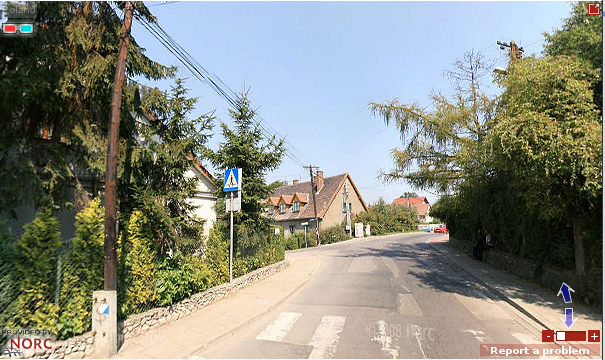
\includegraphics[width=\textwidth]{imgs/image-question21-1}
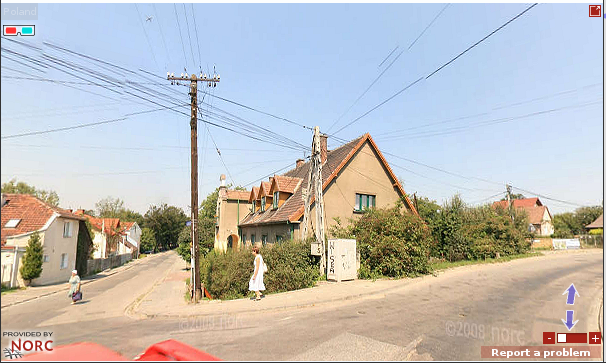
\includegraphics[width=\textwidth]{imgs/image-question21-2}

\begin{itemize}
	\item Do you recognize this point of the city?
	\item If you recognize it, where should you go in order to reach the destination you saw in the video?
\end{itemize}

\newpage

\subsection{Question 2.2}

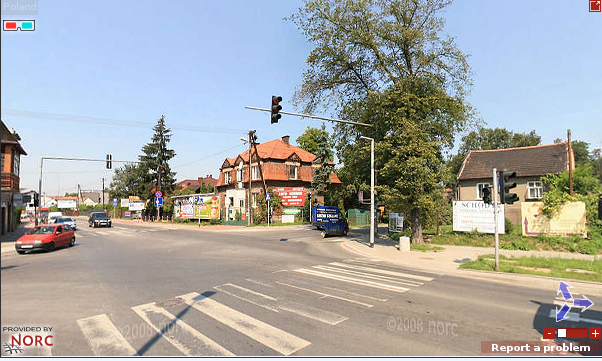
\includegraphics[width=\textwidth]{imgs/image-question22-1}
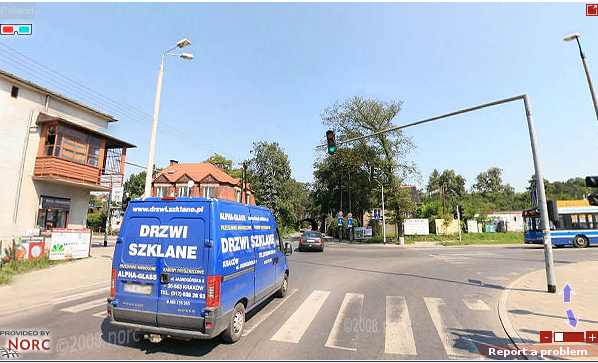
\includegraphics[width=\textwidth]{imgs/image-question22-2}

\begin{itemize}
	\item Do you recognize this point of the city?
	\item If you recognize it, where should you go in order to reach the destination you saw in the video?
\end{itemize}

\newpage

\subsection{Question 2.3}

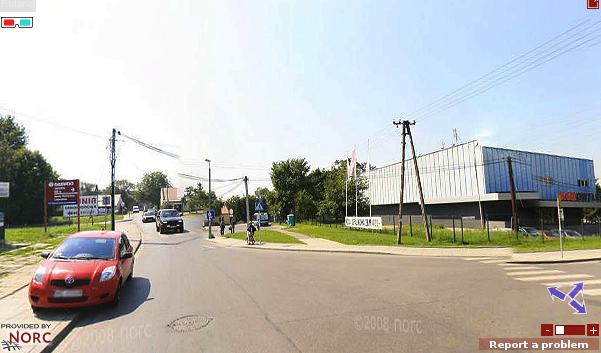
\includegraphics[width=\textwidth]{imgs/image-question23-1}
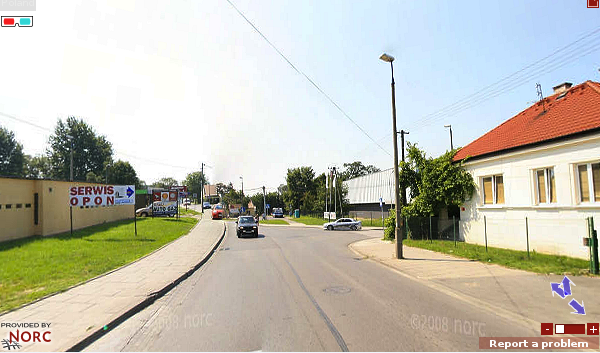
\includegraphics[width=\textwidth]{imgs/image-question23-2}

\begin{itemize}
	\item Do you recognize this point of the city?
	\item If you recognize it, where should you go in order to reach the destination you saw in the video?
\end{itemize}

\newpage

\subsection{Question 3.1}

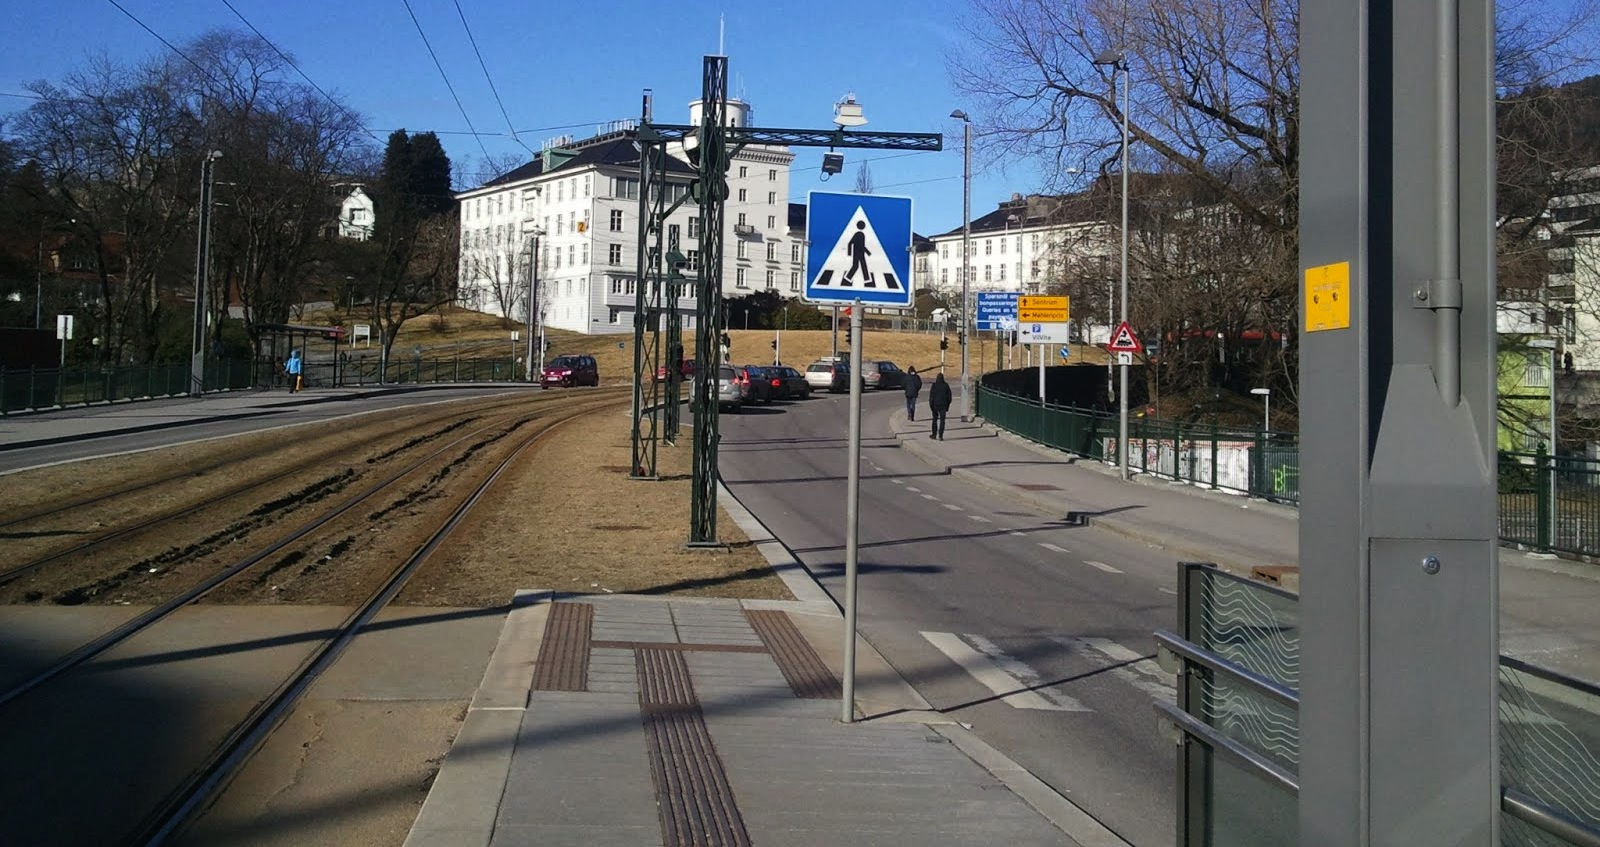
\includegraphics[width=\textwidth]{imgs/image-question31-1}
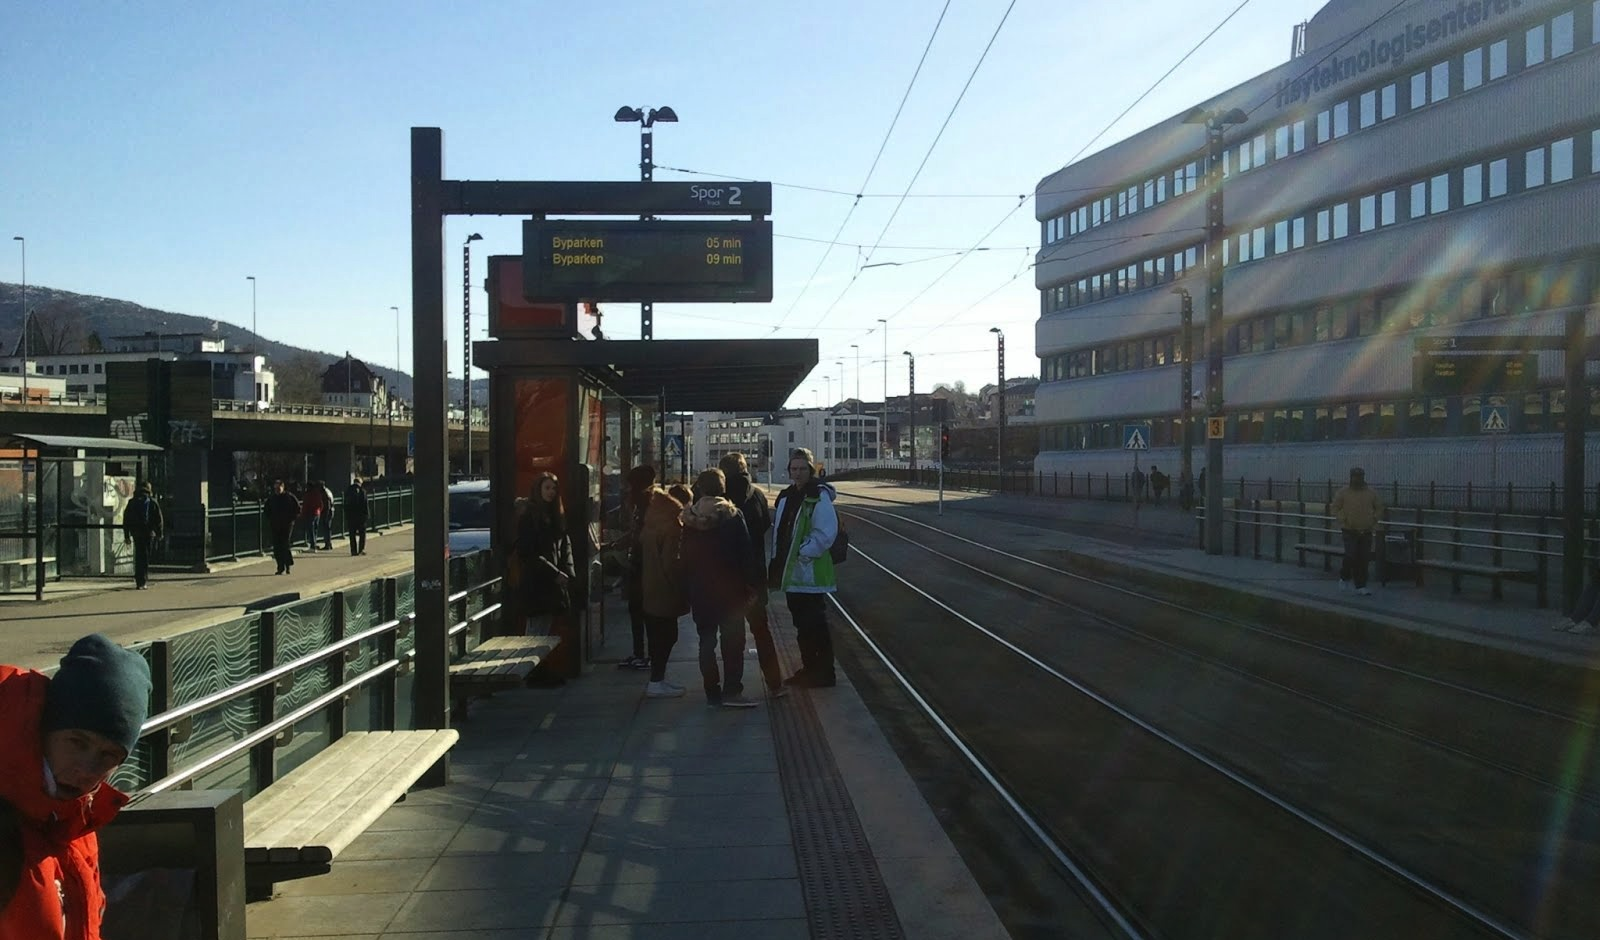
\includegraphics[width=\textwidth]{imgs/image-question31-2}

\begin{itemize}
	\item Do you recognize this point of the city?
	\item If you recognize it, where should you go in order to reach the destination you saw in the video?
\end{itemize}

\newpage

\subsection{Question 3.2}

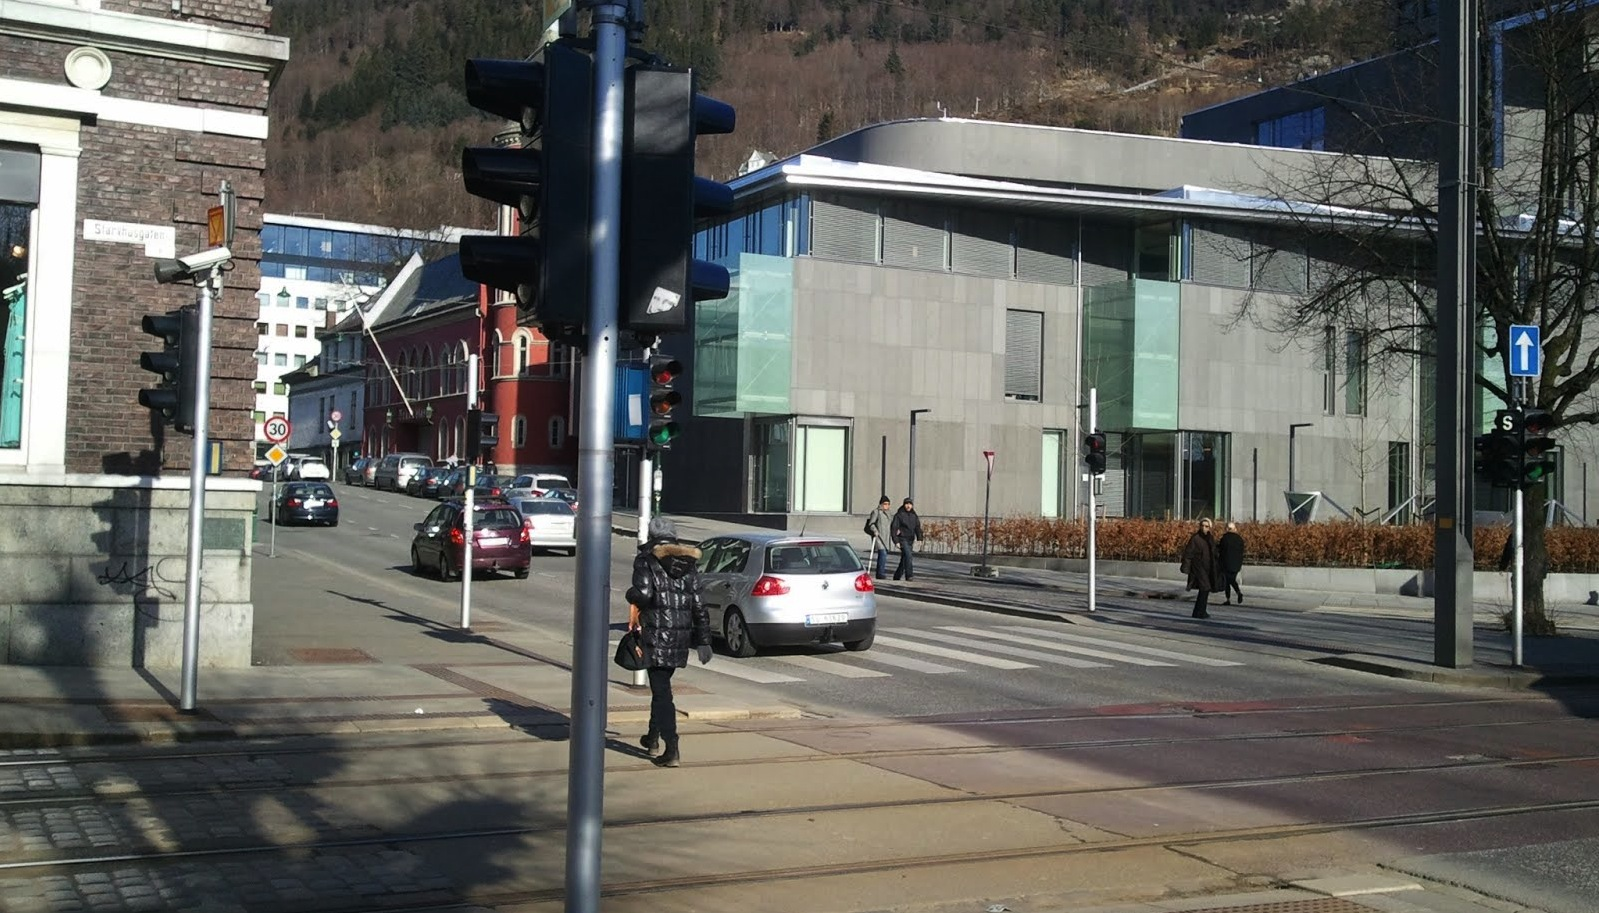
\includegraphics[width=\textwidth]{imgs/image-question32-1}
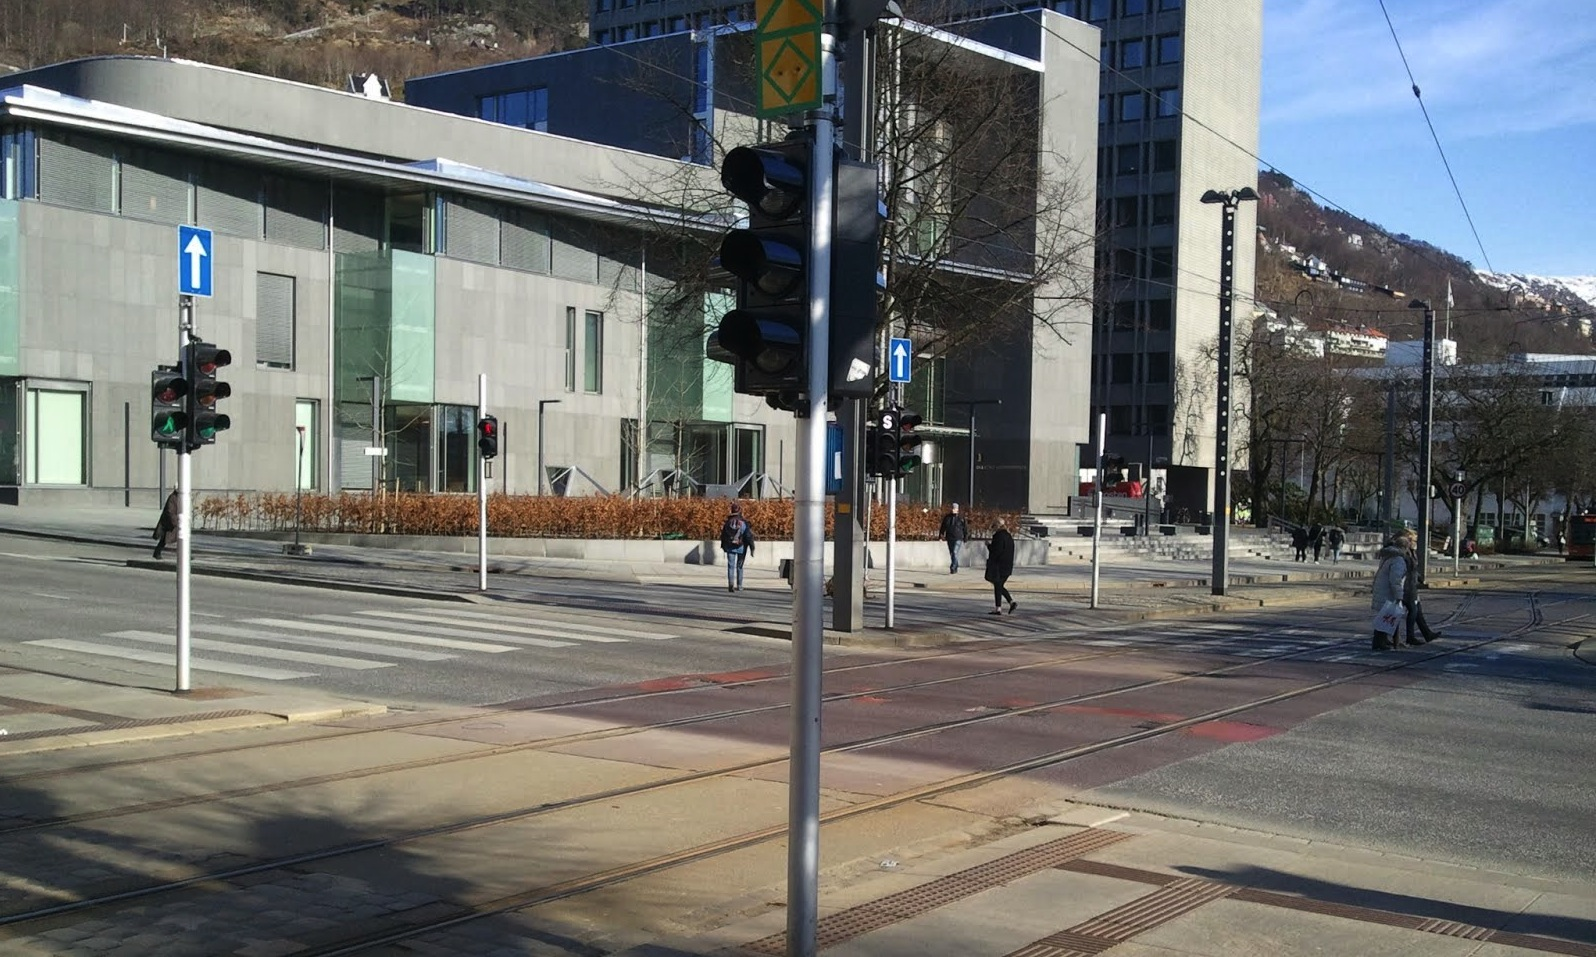
\includegraphics[width=\textwidth]{imgs/image-question32-2}

\begin{itemize}
	\item Do you recognize this point of the city?
	\item If you recognize it, where should you go in order to reach the destination you saw in the video?
\end{itemize}

\newpage

\subsection{Question 3.3}

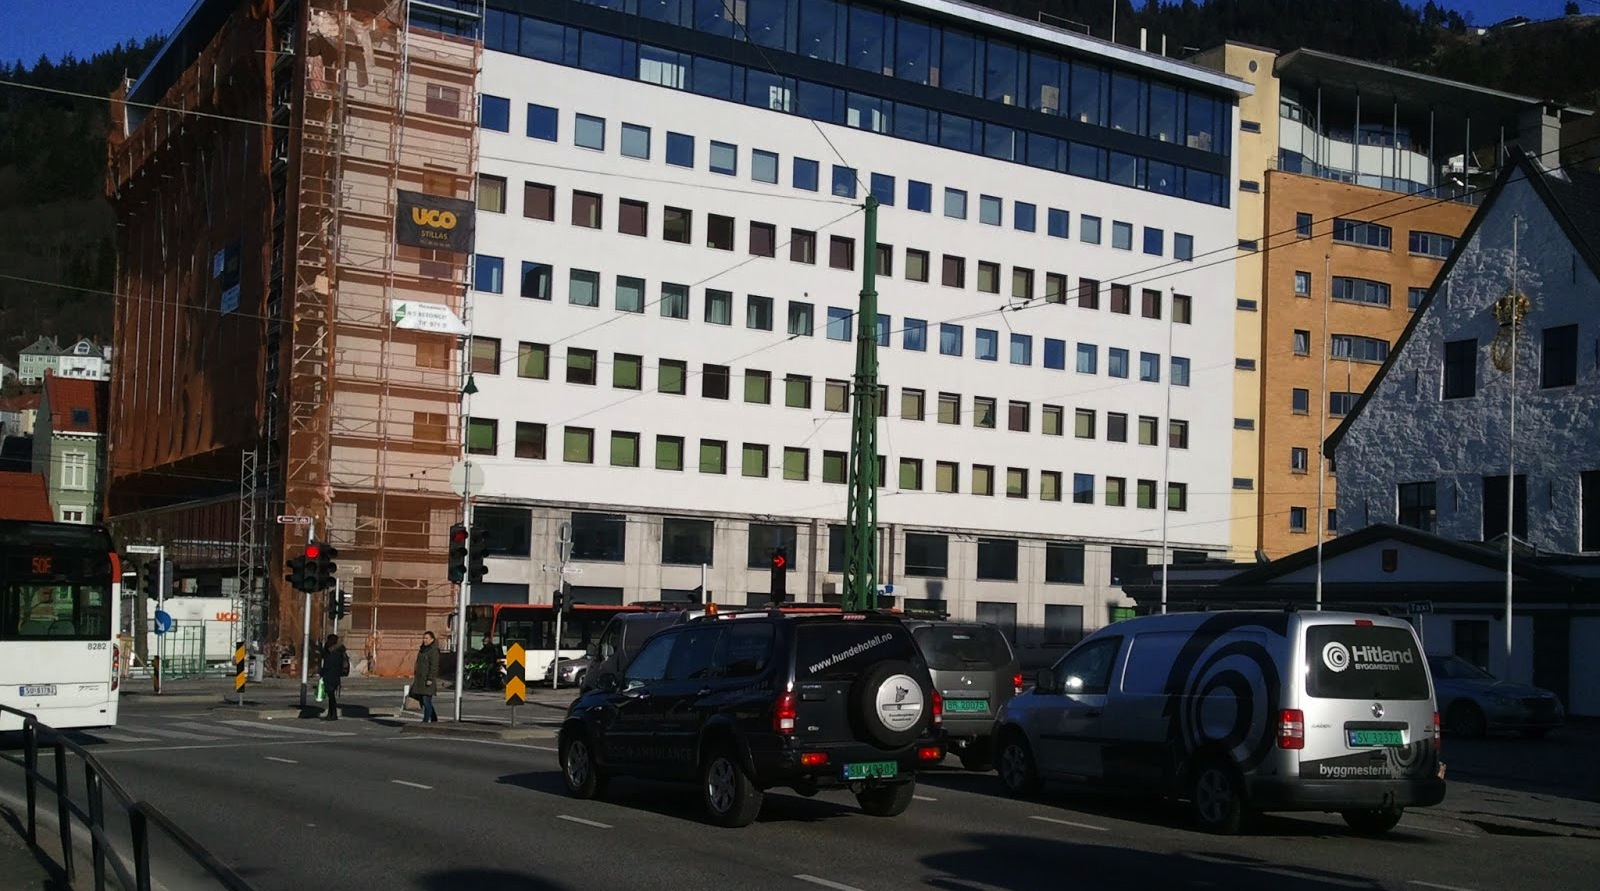
\includegraphics[width=\textwidth]{imgs/image-question33-1}
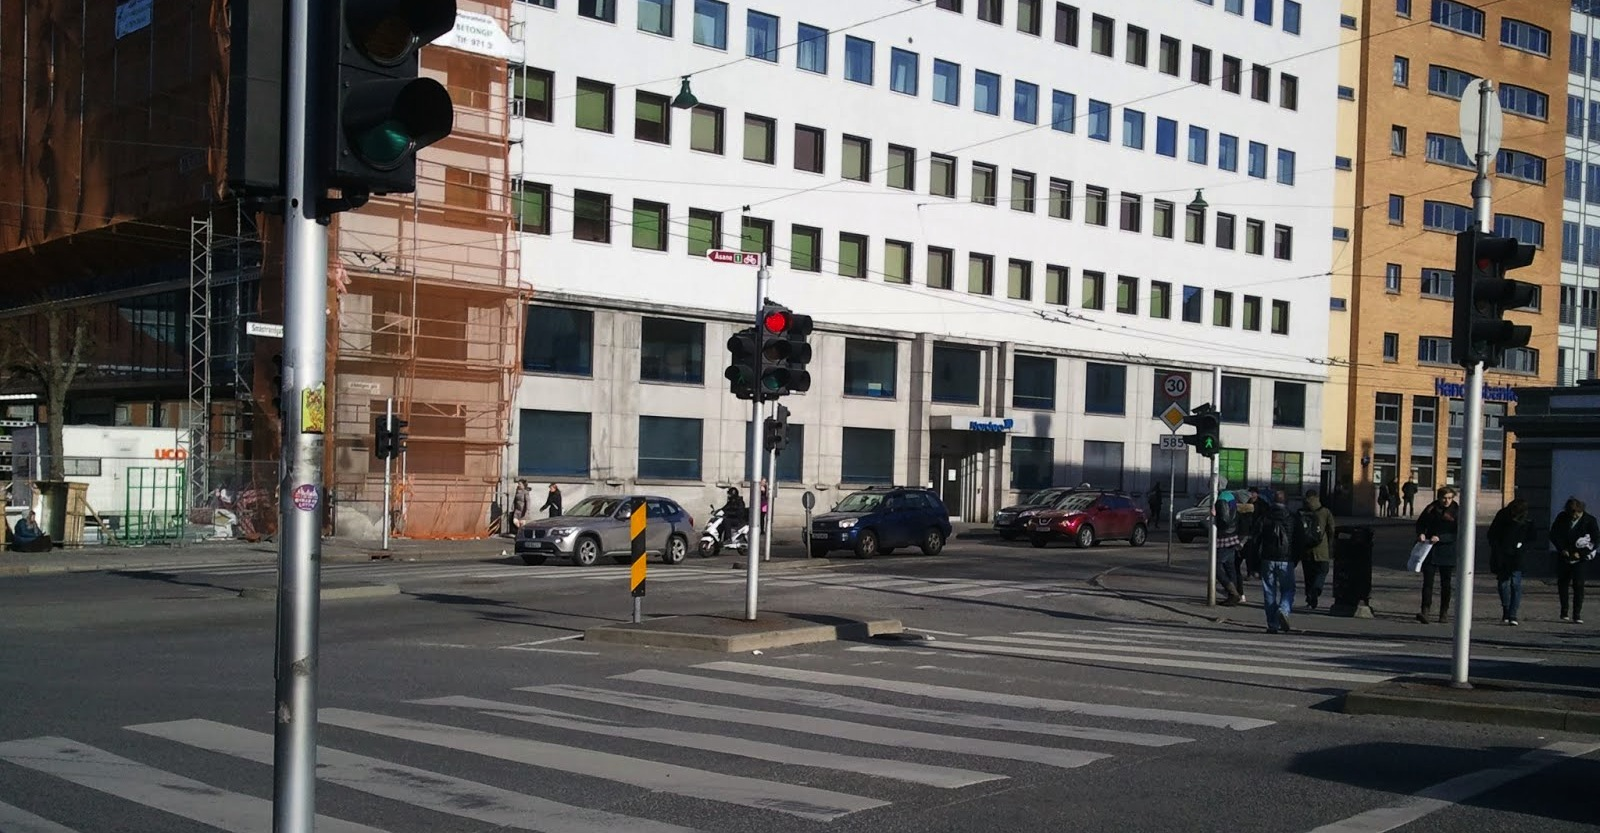
\includegraphics[width=\textwidth]{imgs/image-question33-2}

\begin{itemize}
	\item Do you recognize this point of the city?
	\item If you recognize it, where should you go in order to reach the destination you saw in the video?
\end{itemize}

\newpage


%\section{Results}

%\begin{adjustwidth}{-1cm}{}
%\small
%\begin{center}
%    \begin{tabular}{| l | l | p{2cm} | l | l | l | l | l | l |}
%    \hline
%	& 1 & 2 & 3 & 4 & 5 & 6 & 7 & 8 \\ \hline
%	starting time & 9:21 & 9:52 & 10:28 & 10:28 & 10:42 & 11:02 & 11:15 & 11:15 \\ \hline
%	ending time & 9:34 & 10:01 & 10:32 & 10:32 & 10:50 & 11:10 & 11:23 & 11:23 \\ \hline
%	duration & 13 & 9 & 4 & 4 & 8 & 8 & 8 & 8 \\ \hline
%	re-watched & 0+1+0 & 2+1 & 0+0 & 0+0 & 0+2 & 1+1 & 1+1 & 1+1 \\ \hline
%	% of path reviewed & 100 & 100 & 0 & 0 & 100 & 100 & 100 & 100 \\ \hline
%	score & 0.41 & 0.33 & 0.44 & 0.33 & 0 & 0 & 0.11 & 0.22 \\ \hline
%	confidence speed & 9.62 & 3.7 & 8.3 & 8.3 & 4.2 & 4.2 & 4.2 & 4.2 \\ \hline
%	sex & M & F & M & M & M & F & M & M \\ \hline
%	age & 31 & 24 & 21 & 28 & 53 & 21 & 23 & 23 \\ \hline
%	nationality & Bangladesh & Czech republic & Spain & Spain & Germany & Spain & Ghana & %Spain \\ \hline
%    \end{tabular}
%\end{center}
%\normalsize
%\end{adjustwidth}

%Commenti relativi alla prima parte (visualizzazione del video):

%\begin{itemize}
%	\item Il video è troppo frammentario, è impossibile da capire
%	\item Oddio, dove sono finito? (in risposta ad un fotogramma erroneo lungo il %percorso)
%\end{itemize}

%Commenti relativi alla seconda parte (compilazione del test):

%\begin{itemize}
%	\item Mi sembra di aver visto questa strada ma non ne sono sicuro.
%	\item Ricordo questo incrocio ma non mi ricordo di questo semaforo, non sono sicuro %che sia lo stesso incrocio che ho visto nel video.
%\end{itemize}


%Bibliografia%---------------------------------------------------------------
\bibliographystyle{unsrt}
\addcontentsline{toc}{chapter}{\refname}\nocite{*}
\bibliography{text}
%----------------------------------------------------------------------------

\end{document}